%%%%%%%%%%%%%%%%%%%%%%%%%%%%%%%%%%%%%%%%%%%%%%%%%%%%%%%%%%%%%%%%%%%%%%%%%%%%%%%%
%2345678901234567890123456789012345678901234567890123456789012345678901234567890
%        1         2         3         4         5         6         7         8

% \documentclass[letterpaper, 10 pt, conference]{ieeeconf}  % Comment this line out if you need a4paper

\documentclass[a4paper, 10pt, conference]{ieeeconf}      % Use this line for a4 paper

\IEEEoverridecommandlockouts                              % This command is only needed if 
                                                          % you want to use the \thanks command

\overrideIEEEmargins                                      % Needed to meet printer requirements.

%In case you encounter the following error:
%Error 1010 The PDF file may be corrupt (unable to open PDF file) OR
%Error 1000 An error occurred while parsing a contents stream. Unable to analyze the PDF file.
%This is a known problem with pdfLaTeX conversion filter. The file cannot be opened with acrobat reader
%Please use one of the alternatives below to circumvent this error by uncommenting one or the other
%\pdfobjcompresslevel=0
%\pdfminorversion=4

% See the \addtolength command later in the file to balance the column lengths
% on the last page of the document

% The following packages can be found on http:\\www.ctan.org
\usepackage{graphics} % for pdf, bitmapped graphics files
\usepackage{epsfig} % for postscript graphics files
%\usepackage{mathptmx} % assumes new font selection scheme installed
%\usepackage{times} % assumes new font selection scheme installed
%\usepackage{amsmath} % assumes amsmath package installed
%\usepackage{amssymb}  % assumes amsmath package installed
\title{\LARGE \bf
Human-robot interaction with autonomous vehicles
}
\begin{document}
\maketitle
\thispagestyle{empty}
\pagestyle{empty}


%%%%%%%%%%%%%%%%%%%%%%%%%%%%%%%%%%%%%%%%%%%%%%%%%%%%%%%%%%%%%%%%%%%%%%%%%%%%%%%%
\begin{abstract}
In this report, we will analysis human-robot interaction(HRI) system in three aspects, developer-robot interaction, user-self-driving cars(SDC) interaction and pedestrian-SDC interaction. 
\end{abstract}


%%%%%%%%%%%%%%%%%%%%%%%%%%%%%%%%%%%%%%%%%%%%%%%%%%%%%%%%%%%%%%%%%%%%%%%%%%%%%%%%
\section{INTRODUCTION}
Improvements of SDC technology in the last decade makes autonomous driving gone from “maybe possible” to “definitely possible”. These new capabilities will have profound global impacts that could markedly change society, not to mention the significant improvements they bring to the overall efficiency, convenience, and safety of our roadways and transportation systems\cite{sdc}. To take place of normal car on the road, autonomous vehicles should be able to do all the things a normal car with driver can do. A normal car with driver on the road have lots of interactive with people. According to facial expression and hand gesture, people want to cross the road will understand if it is safe to cross now. Passenger knows where they are going, why the car stops now, how long it takes to arrive destination by communicate with driver. Autonomous vehicles do not have driver. It is driver itself. So SDC should have same communication with people like driver can do. That’s why we need HRI system.

In this report, we separate people HRI need to communicate with into three groups to analysis HRI system. The first one is developers. It is important to feedback vehicles status to developers so that they can improve performance of the autonomous vehicles. Second group is user, people sitting in the car had to believe the car they are taking can successfully send them to their destination. HRI is to help passengers believe it is safe in this vehicle. Third one is pedestrian. HRI also need to let pedestrian and other vehicles know what the car coming is going to do.

\section{Developer-robot interaction}

In traditional car manufacturing industry, test drivers assess vehicle performance for manufacturers. In order to make SDC perform better, therefore, they need to be able to take advantage of human skills and to benefit from human advice and expertise. We can use collaborative control system for teleoperation. Instead of a supervisor dictating to a subordinate, the human and the robot engage dialogue to exchange ideas, to ask questions, and to resolve differences\cite{c2}. Take Fig.\ref{detector} as example. The figure shows a robot module that detect motion from a stream of camera images. As the robot see the image difference, it will notify user and wait for user. Then take action as the user response.
\begin{figure}
    \centering
    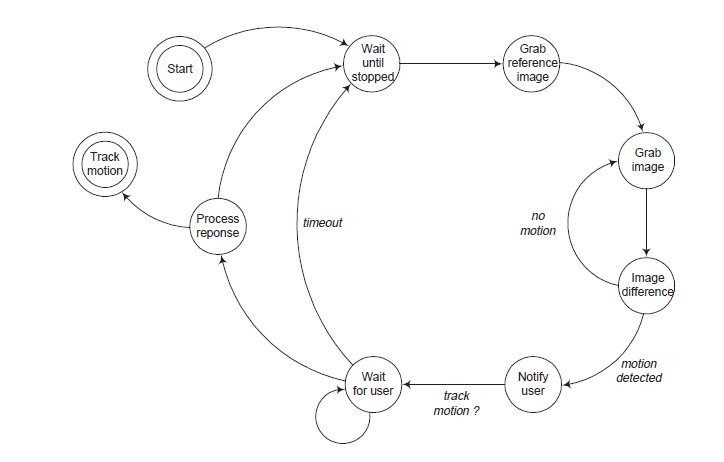
\includegraphics[scale=0.5]{hr-interation.png}
    \caption{Motion Detector state machine\cite{c3}}
    \label{detector}
\end{figure}

To build a collaborative control system, the robot must have self-awareness\cite{c2}. introduce four kinds of features SDC should have. First, it is capable of detecting limitations, determining if it should ask for help, and recognizing when it has to solve problems on its own. Second, the robot must be self-reliant which means it can avoiding hazards, monitoring its health, taking action to be safe when necessary when there is no developer provide accurate information. Third, the system must support dialogue. Developer can communicate effectively with SDC. SDC must be able to ask questions and to judge the quality of responses received. At last, the system must be adaptive. The robot has to be able to adjust its behavior as needed, e.g., asking different questions when it needs designer to answer.

\section{User-SDC interaction}

Some experts predict that we can save millions of lives and grant mobility to all just by removing humans from the driver’s seat. But the difference between theory and practice comes down to this: People are downright scared of robot cars. In fact, a recent AAA study found that 75 percent of Americans are afraid to ride in self-driving cars\cite{wwybr}.
\begin{figure}
    \centering
    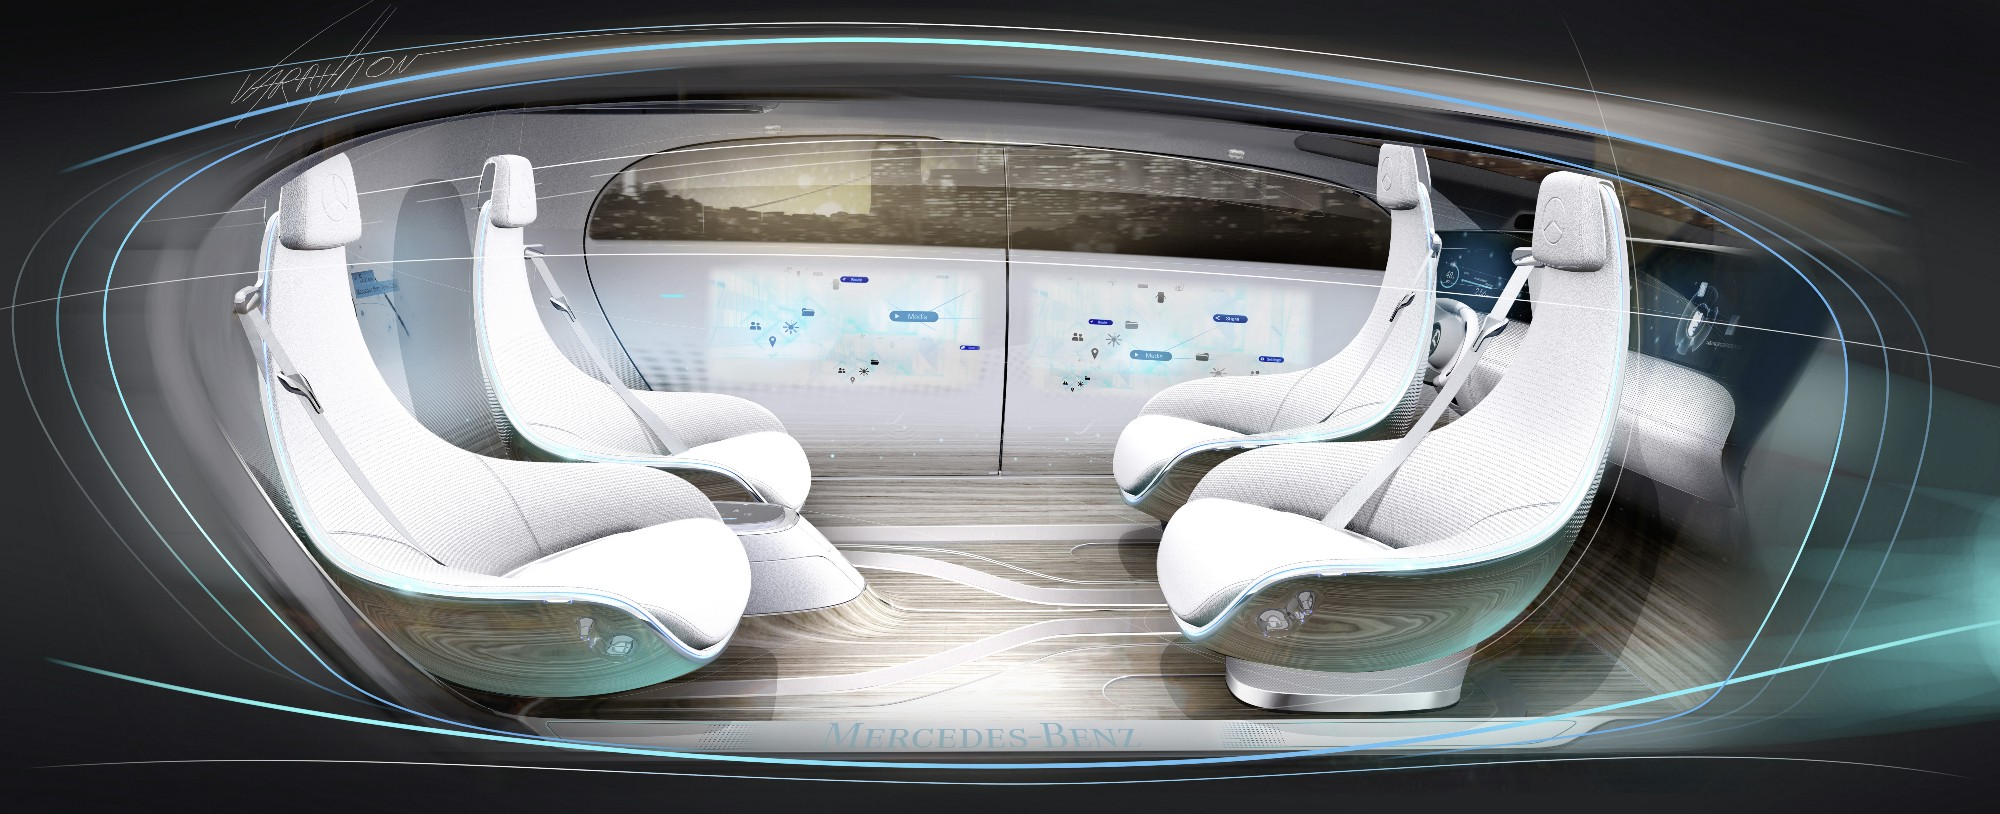
\includegraphics[scale=0.1]{selfdrivingcar.jpeg}
    \caption{An interior concept created by Mercedes-Benz}
    \label{self-driving-car}
\end{figure}
Intel invited some consumers who had no previous driverless car experience to study their feeling of five actions including requesting a vehicle, starting a trip, making changes to the trip, handling errors and emergencies, and pulling over and exiting. In the report, they identified seven areas of tension. We will take some of them as example to introduce how HRI reduce those anxiety. First, people were concerned about the ability of autonomous vehicle handle nuanced situations. Second, passenger feeling some of the alerts and communications might be bothersome. Third, understanding how the technology functions works. Fourth, people wondered if they could use their own voice to communicate with the car, especially if needing to make a detour, change destination, or take off right now. As to the first, third, and fourth problem people concerned. We can show Norman’s seven stages of interaction\cite{cednsd} to passengers. These seven stages are iterated until the intention and goal achieved or the user decides that the intention or goal has to be modified\cite{tehri}. With those information, people will understand how the car works. With understanding how car works, they feel more comfortable with the autonomous car. For example, when slowing down or accelerating, show in the LED screen there is a stop sign ahead so we slow down now or we are entering the highway so we accelerate.

Self-driving car will have totally new seats arrangement. The screen in the car will be much bigger than traditional car. Like Fig.\ref{self-driving-car} shows, people will face to each other in the car. There will be more room for designer to decide what should be shown to user and where the information should show up depends on how important the information is.


\section{Pedestrian-SDC interaction}

\begin{figure}
    \centering
    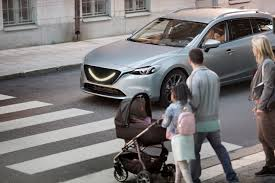
\includegraphics[scale=0.8]{smilecar.jpg}
    \caption{smiling self-driving car(Jeremy Hsu Sep 2016)}
    \label{smile car}
\end{figure}

There is a huge amount of unspoken interactions between drivers and the world around them. Gesturing to a pedestrian to cross the street, horn to warning other driver get into one-way street in wrong direction. It’s important for SDC to engage in that interactions as well. Drive.ai is working on LED signs on the vehicle that use text and emoji-like pictures to communicate. They also working on auditory feedback too. The team think horns do not change direction or volume which is bad. They are working on an advanced version of its auditory feedback, allowing the car to "see the context" of the situation and emit a "more socially appropriate" honk. In \cite{google}, Google reveals that it's been training the cars to honk at the absent-minded humans around them when the situation demands. If another vehicle is slowly reversing towards us, we might sound two short, quieter pips as a friendly heads up to let the driver know we're behind. However, if there's a situation that requires more urgency, we'll use one loud sustained honk\cite{google}. As in the Fig.\ref{smile car} shows. SEMCON working on The Smiling Car system when the self-driving car’s sensors detect a pedestrian, a signal is sent to a display at the front and a smile lights up that confirms that the car will stop for the pedestrian. The team use cameras with systems for eye tracking technology, so SDC read a gaze directed toward the car then provide immediate feedback through a smile lighting up on the grille.

\section{Conclusion}
HRI have different systems for different people. When interact with designer, the system should have ability to show the problem vehicle met and execute designer’s command. Interact with pedestrian just need to show people what the car is doing and going to do. User is more complicate, the system need to be able to execute user’s command like designer do, also, the system should show lot of information about the car and road situation to let user know all the things is in control.

%%%%%%%%%%%%%%%%%%%%%%%%%%%%%%%%%%%%%%%%%%%%%%%%%%%%%%%%%%%%%%%%%%%%%%%%%%%%%%

\addtolength{\textheight}{-12cm}   % This command serves to balance the column lengths
                                  % on the last page of the document manually. It shortens
                                  % the textheight of the last page by a suitable amount.
                                  % This command does not take effect until the next page
                                  % so it should come on the page before the last. Make
                                  % sure that you do not shorten the textheight too much.

%%%%%%%%%%%%%%%%%%%%%%%%%%%%%%%%%%%%%%%%%%%%%%%%%%%%%%%%%%%%%%%%%%%%%%%%%%%%%%%

\begin{thebibliography}{99}

\bibitem{sdc} M. Daily, S. Medasani, R. Behringer and M. Trivedi, "Self-Driving Cars," in Computer, vol. 50, no. 12, pp. 18-23, 2017. 
\bibitem{c2} Fong, Terrence, Charles Thorpe, and Charles Baur. "Collaboration, dialogue, human-robot interaction." Robotics Research. Springer, Berlin, Heidelberg, 2003. 255-266.
\bibitem{c3} Fong, Terrence, Charles Thorpe, and Charles Baur. Collaborative control: A robot-centric model for vehicle teleoperation. Vol. 1. Carnegie Mellon University, The Robotics Institute, 2001.
\bibitem{wwybr} https://newsroom.intel.com/editorials/when-will-you-be-ready-get-driverless-car/ August 24, 2017
\bibitem{rcmvt} Fong T (2001) Collaborative control: a robot-centric model for vehicle teleoperation. PhD thesis, Carnegie Mellon University, Pittsburgh. CMU-RI-TR-01-34.
\bibitem{cednsd} Norman, D. 1986. Cognitive Engineering in Donald Norman and Stephen Draper (Eds) User-centered design: new perspectives on human-computer interaction, Erlbaum Associates: Hillsdale, N.J, 31-62.
\bibitem{tehri} Scholtz, Jean. "Theory and evaluation of human robot interactions." System Sciences, 2003. Proceedings of the 36th Annual Hawaii International Conference on. IEEE, 2003.


\bibitem{google} Google Self-Driving Car Project Monthly Report May 2016 https://static.googleusercontent.com/media/www.google.com/en//selfdr ivingcar/files/reports/report-0516.pdf


\end{thebibliography}

\end{document}
